% \subsection{Definição das variáveis de controle}
% \label{sec:var_controle}

% Para este trabalho, estabeleceu-se um conjunto de variáveis, elas contém a posição e velocidade do perseguidor no referencial ECI e \gls{lvlh}, além de sua atitude e as velocidades das juntas do \gls{mr}, entre outras.

% \subsubsection{Variáveis no referencial ECI}
% O vetor de estados reúne as 19 variáveis necessárias para descrever completamente o movimento da espaçonave perseguidora e do manipulador robótico acoplado, conforme a Tabela~\ref{tab:vetor_estados}.

% \begin{table}[ht]
% \centering
% \caption{Composição do vetor de estados $\mathbf{x}$ (dimensão total: 19).}
% \label{tab:vetor_estados}
% \begin{tabular}{lll}
% \toprule
% \textbf{Grupo} & \textbf{Variáveis} & \textbf{Descrição} \\ 
% \midrule
% Translacional &
% $\vec{r} = [x, y, z]^T$ &
% Posição \\[2pt]
%  &
% $\vec{v} = [\dot{x}, \dot{y}, \dot{z}]^T$ &
% Velocidade linear \\[3pt]
% Atitude &
% $\mathbf{q} = [q_0, q_1, q_2, q_3]^T$ &
% Quaternion unitário \\[2pt]
%  &
% $\vec{\omega} = [\omega_x, \omega_y, \omega_z]^T$ &
% Velocidade angular \\[3pt]
% Manipulador robótico &
% $\boldsymbol{\theta} = [\theta_1, \theta_2, \theta_3]^T$ &
% Posições articulares \\[2pt]
%  &
% $\dot{\boldsymbol{\theta}} = [\dot{\theta}_1, \dot{\theta}_2, \dot{\theta}_3]^T$ &
% Velocidades articulares \\[2pt]
% \bottomrule
% \end{tabular}
% \end{table}

% As variáveis translacionais $\vec{r}$ e $\vec{v}$ representam a posição e a velocidade do do centro de massa da \gls{emtr} em relação a origem do \gls{lvlh}, definido no alvo, e são utilizadas na formulação da dinâmica da espaçonave nas versões de movimento absoluto (ECI) e movimento relativo \gls{lvlh} entre o perseguidor e o alvo.

% O conjunto $\{\vec{q},\,\vec{\omega}\}$ a posição e a velocidade angular associados ao movimento de atitude da espaçonave.  
% O quaternion $\vec{q}$ fornece a orientação do corpo em relação ao alvo, sendo utilizado na integração das equações cinemáticas de atitude.  
% Por sua vez, a velocidade angular $\vec{\omega}$ é utilizada tanto na equação de Euler quanto na formulação Lagrangeana, sendo as componentes do vetor de rotação instantânea do corpo.


% Por fim, as variáveis $\vec{\theta}$ e $\dot{\vec{\theta}}$ descrevem o estado articular do \gls{mr}. São usados nas equações cinemáticas e dinâmicas do manipulador, influenciando na variação temporal do tensor de inércia total da espaçonave e o acoplamento dinâmico entre base e elos. Sendo assim, o vetor de estados fornece um conjunto estados capaz de alimentar tanto a dinâmica de Euler (modo não-operacional do manipulador robótico) quanto a de Lagrange (modo acoplado base--manipulador robótico).

% \subsubsection{Variáveis de controle}
% As variáveis de controle listadas na Tabela~\ref{tab:torques_aceleracoes} representam as grandezas atuantes e resultantes nas equações dinâmicas da espaçonave perseguidora.  

% \begin{table}[ht]
% \centering
% \caption{Variáveis de controle e resposta dinâmica.}
% \label{tab:torques_aceleracoes}
% \begin{tabular}{lll}
% \toprule
% \textbf{Tipos de controle} & \textbf{Símbolo} & \textbf{Descrição} \\ 
% \midrule
% Controle de atitude & $\vec{\tau}_{base}$ & Torques aplicados à base \\[2pt]
%  & $\dot{\vec{\omega}}$ & Acelerações angulares resultantes \\[3pt]
% Controle das juntas & $\vec{\tau}_{juntas}$ & Torques nas juntas do MR \\[2pt]
%  & $\ddot{\boldsymbol{\theta}}$ & Acelerações articulares resultantes \\[2pt]
% \bottomrule
% \end{tabular}
% \end{table}

% Os torques $\vec{\tau}_{\text{atitude}}$ e $\vec{\tau}_{\text{juntas}}$ constituem as entradas de controle do sistema, produzidas pelos controladores PD de atitude e de juntas, respectivamente.  
% Esses torques são aplicados à base e aos elos do manipulador robótico e correspondem às forças efetivas responsáveis pela geração de movimento rotacional no sistema acoplado.
% As acelerações $\dot{\vec{\omega}}_{\text{base}}$ e $\ddot{\vec{\theta}}$ são obtidas como saídas diretas das equações diferenciais de movimento, derivadas a partir da formulação de Euler ou de Lagrange.  
% Enquanto a dinâmica de Euler considera apenas o movimento de atitude da base (sem acoplamento com o \gls{mr}), a formulação de Lagrange incorpora os efeitos de inércia cruzada, permitindo calcular as acelerações da base e das juntas de forma simultânea.
% A relação entre torques e acelerações é mediada pela matriz de inércia generalizada $\mathbf{M}(\mathbf{q})$ e pelos termos de Coriolis e centrífuga $\mathbf{C}(\mathbf{q}, \dot{\mathbf{q}})$, segundo a equação matricial

% \begin{equation}
% \mathbf{M}(\mathbf{q})\,\ddot{\mathbf{q}} + \mathbf{C}(\mathbf{q}, \dot{\mathbf{q}}) = \boldsymbol{\tau},
% \label{eq:lagrange_forma_compacta}
% \end{equation}

% onde $\ddot{\mathbf{q}} = [\dot{\vec{\omega}}_{\text{base}}^T,\, \ddot{\boldsymbol{\theta}}^T]^T$ é o vetor de acelerações generalizadas e $\boldsymbol{\tau} = [\boldsymbol{\tau}_{\text{atitude}}^T,\, \boldsymbol{\tau}_{\text{juntas}}^T]^T$ o vetor de torques aplicados.  
% Dessa forma, as variáveis de controle estão diretamente associadas à excitação dinâmica do sistema, determinando sua resposta em atitude e nas articulações do manipulador.
% O modelo dinâmico considerado integra diferentes subsistemas, como:
% \begin{enumerate}[label=(\roman*)]
%     \item as equações de \gls{hcw} linearizadas para a descrição do movimento relativo;
%     \item as equações de atitude baseadas na cinemática dos quaternions;
%     \item a dinâmica do corpo rígido de Euler;
%     \item a dinâmica acoplada de Lagrange;
%     \item a dinâmica do \gls{mr} acoplado à base da espaçonave.
% \end{enumerate}

\subsection{Definição das variáveis de controle}
\label{sec:var_controle}

Para este trabalho, estabeleceu-se um conjunto de variáveis, elas contém a posição e velocidade do perseguidor no referencial ECI e \gls{lvlh}, além de sua atitude e as velocidades das juntas do \gls{mr}, entre outras.

\subsubsection{Variáveis no referencial LVLH}
\label{sec:var_ref_lvlh}

Na fase de aproximação de curta distância, a dinâmica de translação relativa é formulada no referencial \gls{lvlh} centrado no alvo.
Nesse referencial, o perseguidor tem sua posição e velocidade relativas ao alvo e constituem o estado utilizado pelo modelo de \gls{hcw} e pela lei de controle de translação.

Define-se o vetor de posição relativa do perseguidor em relação ao alvo no LVLH por

\begin{equation}
\vec r_{\text{rel}}
=
\begin{bmatrix}
x \\[2pt] y \\[2pt] z
\end{bmatrix}_{\text{LVLH}},
\end{equation}

onde $x$ é a componente ao longo da trajetória (\emph{along--track}), $y$ é a componente transversal (\emph{cross--track}) e $z$ é a componente radial.
Por sua vez, a velocidade relativa no LVLH é escrita como

\begin{equation}
\vec v_{\text{rel}}
=
\begin{bmatrix}
\dot x \\[2pt] \dot y \\[2pt] \dot z
\end{bmatrix}_{\text{LVLH}}.
\end{equation}

O vetor de estado empregado no modelo de translação é então organizado como

\begin{equation}
\vec x_{\text{rel}}
=
\begin{bmatrix}
\vec r_{\text{rel}} \\[2pt]
\vec v_{\text{rel}}
\end{bmatrix},
\end{equation}

que contém as grandezas de posição e velocidade relativas no LVLH.
Na simulação computacional, $\vec x_{\text{rel}}$ é obtido a partir das posições e velocidades inerciais do perseguidor e do alvo por meio do bloco de conversão ECI para LVLH.
O bloco Comparador distância relativa (LVLH) fornece ainda a distância relativa escalar

\begin{equation}
\rho = \lVert \vec r_{\text{rel}} \rVert,
\end{equation}

utilizada para monitorar a aproximação do perseguidor no alvo.
As variáveis $\vec r_{\text{rel}}$ e $\vec v_{\text{rel}}$ realimentam a lei de controle de translação, que gera o comando de aceleração de controle no LVLH.
Essa aceleração é aplicada ao modelo de \gls{hcw}, fechando a malha de controle de aproximação de curta distância.

\begin{figure}[H]
\centering
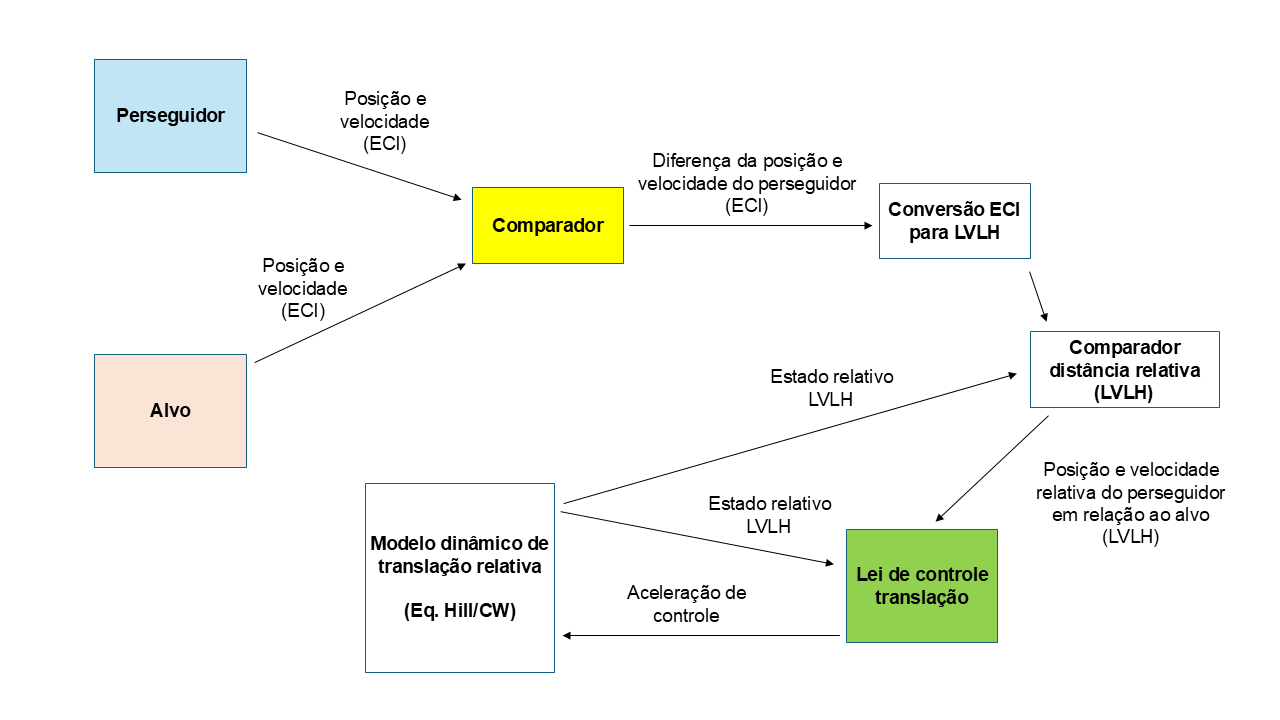
\includegraphics[width=1\linewidth]{3 Formulacao matematica/5 Formulacao problema controle/Imagens formulacao controle/1 Eq Hill CW PD.png}
\caption{Diagrama de blocos da lei de controle da translação do perseguidor.}
    \label{fig:controle_hcw}
\end{figure}

A Figura~\ref{fig:controle_hcw} apresenta o fluxo de sinais da lei de controle de translação do perseguidor durante a aproximação de curta distância.
O vetor de estado relativo $\vec x_{\text{rel}}$ é convertido para o referencial \gls{lvlh}, comparado com a referência de distância relativa e utilizado pela lei de controle para gerar a aceleração de controle $\vec a_{\text{c}}$, aplicada ao modelo de \gls{hcw}.
Essa malha permanece ativa desde o início da aproximação curta até o término da missão de \gls{rvdb}, mantendo a distância relativa entre as espaçonaves dentro de limites especificados para cada fase da missão e para reduzir o risco de colisão ou perda de alinhamento translacional.

\subsubsection{Variáveis de atitude}
\label{sec:var_attde}

Nas fases de aproximação curta e na etapa inicial da aproximação final,
a atitude do perseguidor é ajustada por um controlador de atitude em
três eixos.
Neste momento, o perseguidor obtém a atitude do alvo, que será usada como referência até o final da missão.
Ao mesmo tempo, o comparador interno do perseguidor faz a leitura de sua própria atitude para obter o erro de atitude relativa que alimenta a lei de controle, conforme o diagrama de blocos da
Figura~\ref{fig:controle_attde_euler}.

\begin{figure}[H]
\centering
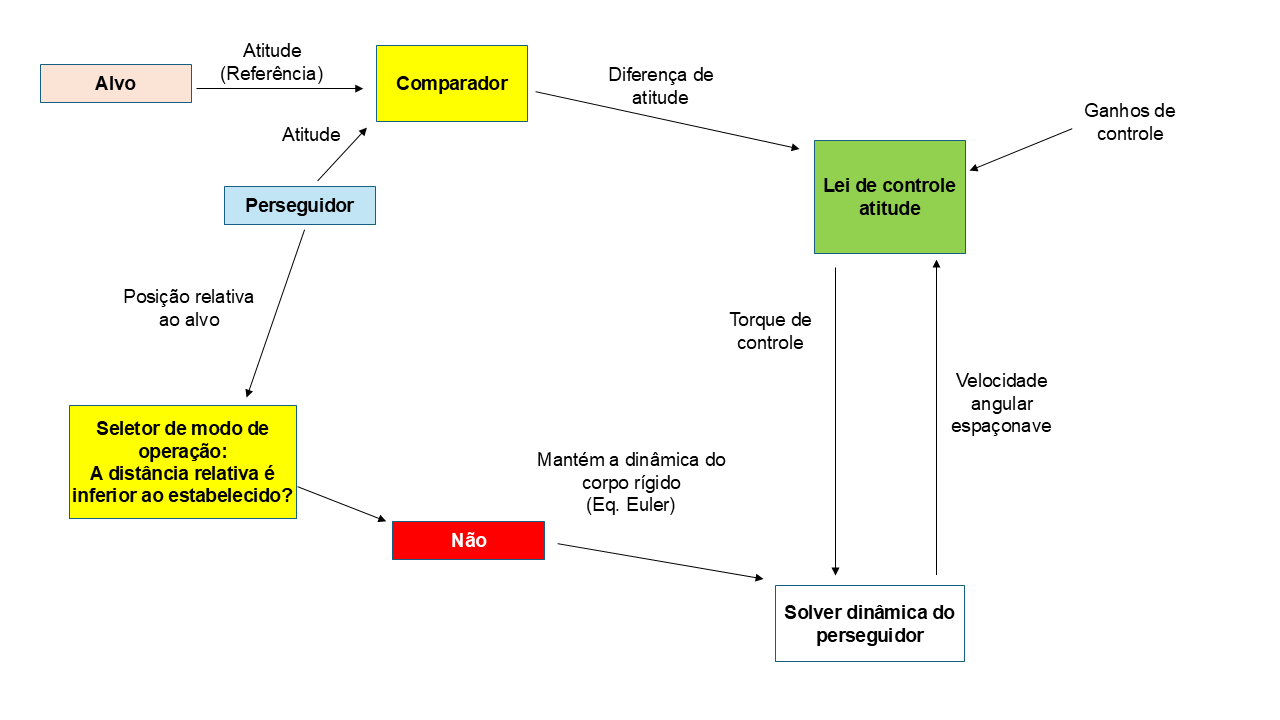
\includegraphics[width=1\linewidth]{3 Formulacao matematica/5 Formulacao problema controle/Imagens formulacao controle/2 Atitude durante Euler.png}
\caption{Diagrama de blocos da lei de controle da atitude do perseguidor.}
    \label{fig:controle_attde_euler}
\end{figure}

A atitude do perseguidor em relação ao referencial inercial é
representada por um quaternion unitário
e pela velocidade angular do corpo

\begin{equation}
{}^{B}\!\vec\omega_B
=
\begin{bmatrix}
\omega_x \\[2pt] \omega_y \\[2pt] \omega_z
\end{bmatrix}.
\end{equation}

A atitude de referência é igualmente escrita por um quaternion
$\vec q_{\text{ref}}$ associado ao alvo no referencial do corpo.
O erro de atitude utilizado na realimentação é definido a partir do
quaternion relativo, conforme a equação \eqref{eq:quat_relativo},
cuja parte vetorial está associada ao eixo de rotação
e ao ângulo equivalente entre as duas atitudes.

O vetor de estado empregado no controle de atitude é organizado como

\begin{equation}
\vec x_{\text{att}}
=
\begin{bmatrix}
\vec q_B \\[2pt]
{}^{B}\!\vec\omega_B
\end{bmatrix},
\end{equation}

enquanto a variável de saída da lei de controle é o torque de controle
aplicado ao corpo da espaçonave.
Esse torque atua como entrada nas equações de Euler do movimento
rotacional da espaçonave, fechando a malha de controle de atitude ao
longo de toda a aproximação curta e da parte inicial da aproximação
final.

\subsubsection{Variáveis do MR}
\label{sec:var_mr}


